\documentclass[12pt,twoside,a4paper]{article}
\usepackage{graphicx}
\graphicspath{ {../img/} }
\usepackage[left=2cm, right=2cm, top=2.5cm, bottom=3cm]{geometry}
\title{Operativni sistem Linux}
\author{Vojislav Lazić}
\date{February 2019}
\begin{document}
    \thispagestyle{empty}
    \noindent
    Šesta beogradska gimanzija\\
    Milana Rakića 33\\
    Beograd
    \vfill
    \begin{center}
        \begin{Large}
        Maturski rad iz informatike\\
        \medskip 
        \end{Large}
        {\Huge
        Operativni sistem Linux}
    \end{center}
    \vfill
    \noindent Mentor: \hfill Učenik:\\
    Olivera Mihailović \hfill Vojislav Lazić IV$_{9}$\\
    Profesor informatike
    \vfill
    \begin{center}
        Beograd, jun 2019.
    \end{center}
\thispagestyle{empty}


\newpage
\tableofcontents
\newpage
\section{Istorija Linuxa}
\indent Za stvaranje Linux-a bilo je potrebno nekoliko komponenti, najvažnija od kojih je Unix. Unix su stvorili Ken Tompson i Denis Riči. Njih dvojica, zajedno sa timom inženjera u Belovim laboratorijama, su radili na Multics sistemu (\textbf{M}ultiplexed \textbf{I}nformation and \textbf{C}omputing \textbf{S}ervice), pravljen sa idejom da bude sistem koji može da radi više poslova u isto vreme. Tompson i Riči su u  tom periodu počeli da rade na svom sopstvenom sistemu, zasnovan na Multics-u, po imenu Unix, prvi put objavljen 1970. godine. Kasnije, kad je C programski jezik, koji je Riči napisao zajedno sa Brajanom Kernigenom, postao dovoljno razvijen, Unix je potpuno prepisan u C-u, što je pomoglo njegovom rasprostranjenju u razne akademske institucije i poslove. Zbog promenljive i prilagodljive prirode Unix-a, razni univerziteti su počeli da prave svoje verzije Unix-a, jedan od najpopularnijih je bio BSD (\textbf{B}erkeley \textbf{S}oftware \textbf{D}istribution), koji je još u upotrebi danas.\\

1983. godine, Ričard Metju Stalman je započeo GNU projekat, namenjen da bude slobodna alternativa za Unix. Do ranih 90-ih, napisano je dovoljno softvera da se napravi citav operativni sistem. Jedino što je nedostajalo je ``kernel'' ili ``jezgro'' operativnog sistema, deo koji bi trebao sve ostale komponente da spoji. GNU je imao, i još ima, u pravljenju svoji kernel, GNU Hurd, ali nikad nije završen. Postojao je i kernel zasnovan na BSD-u, ali bez dovoljno funkcionalnosti.\\

Nedostatak besplatnog i korisnog kernel-a, je nerviralo Linusa Torvaldsa, pa je stoga odlučio da napiše svoji sopstveni. Torvalds je bio upoznat već sa Minix-om i sa GNU softverom i dok je bio student informatike na Univerzitetu u Finskoj je počeo da radi na projektu koji bi kasnije postao Linux kernel. 25.-og avgusta 1991. godine, Torvalds je postavio na Usenet newsgroup-i o svom projektu. Nastavio je da bude projekat na kome je samo on radio, ali s vremenom je steklo sve više pažnje od drugih programera. Danas je preko 15000 programera  doprinelo preko 17 miliona linija koda.
\newpage
\begin{figure}[h]
	\centering
    \subfloat[Ken Tompson i Denis Riči, tvorci UNIX-a]{{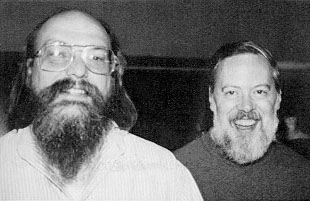
\includegraphics[height=3cm,width=4cm]{d_r} }}
    \hspace{1cm}
    \subfloat[Linus Torvalds, tvorac Linux-a]{{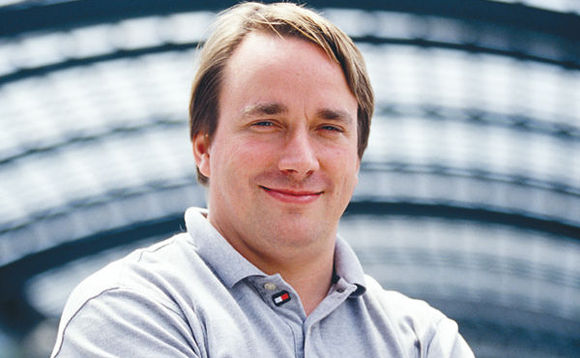
\includegraphics[height=3cm,width=4cm]{linus} }}
\end{figure}
\begin{figure}[h]
	\centering
    \subfloat[Flopi diskovi sa verzijom 0.12 Linux-a]{{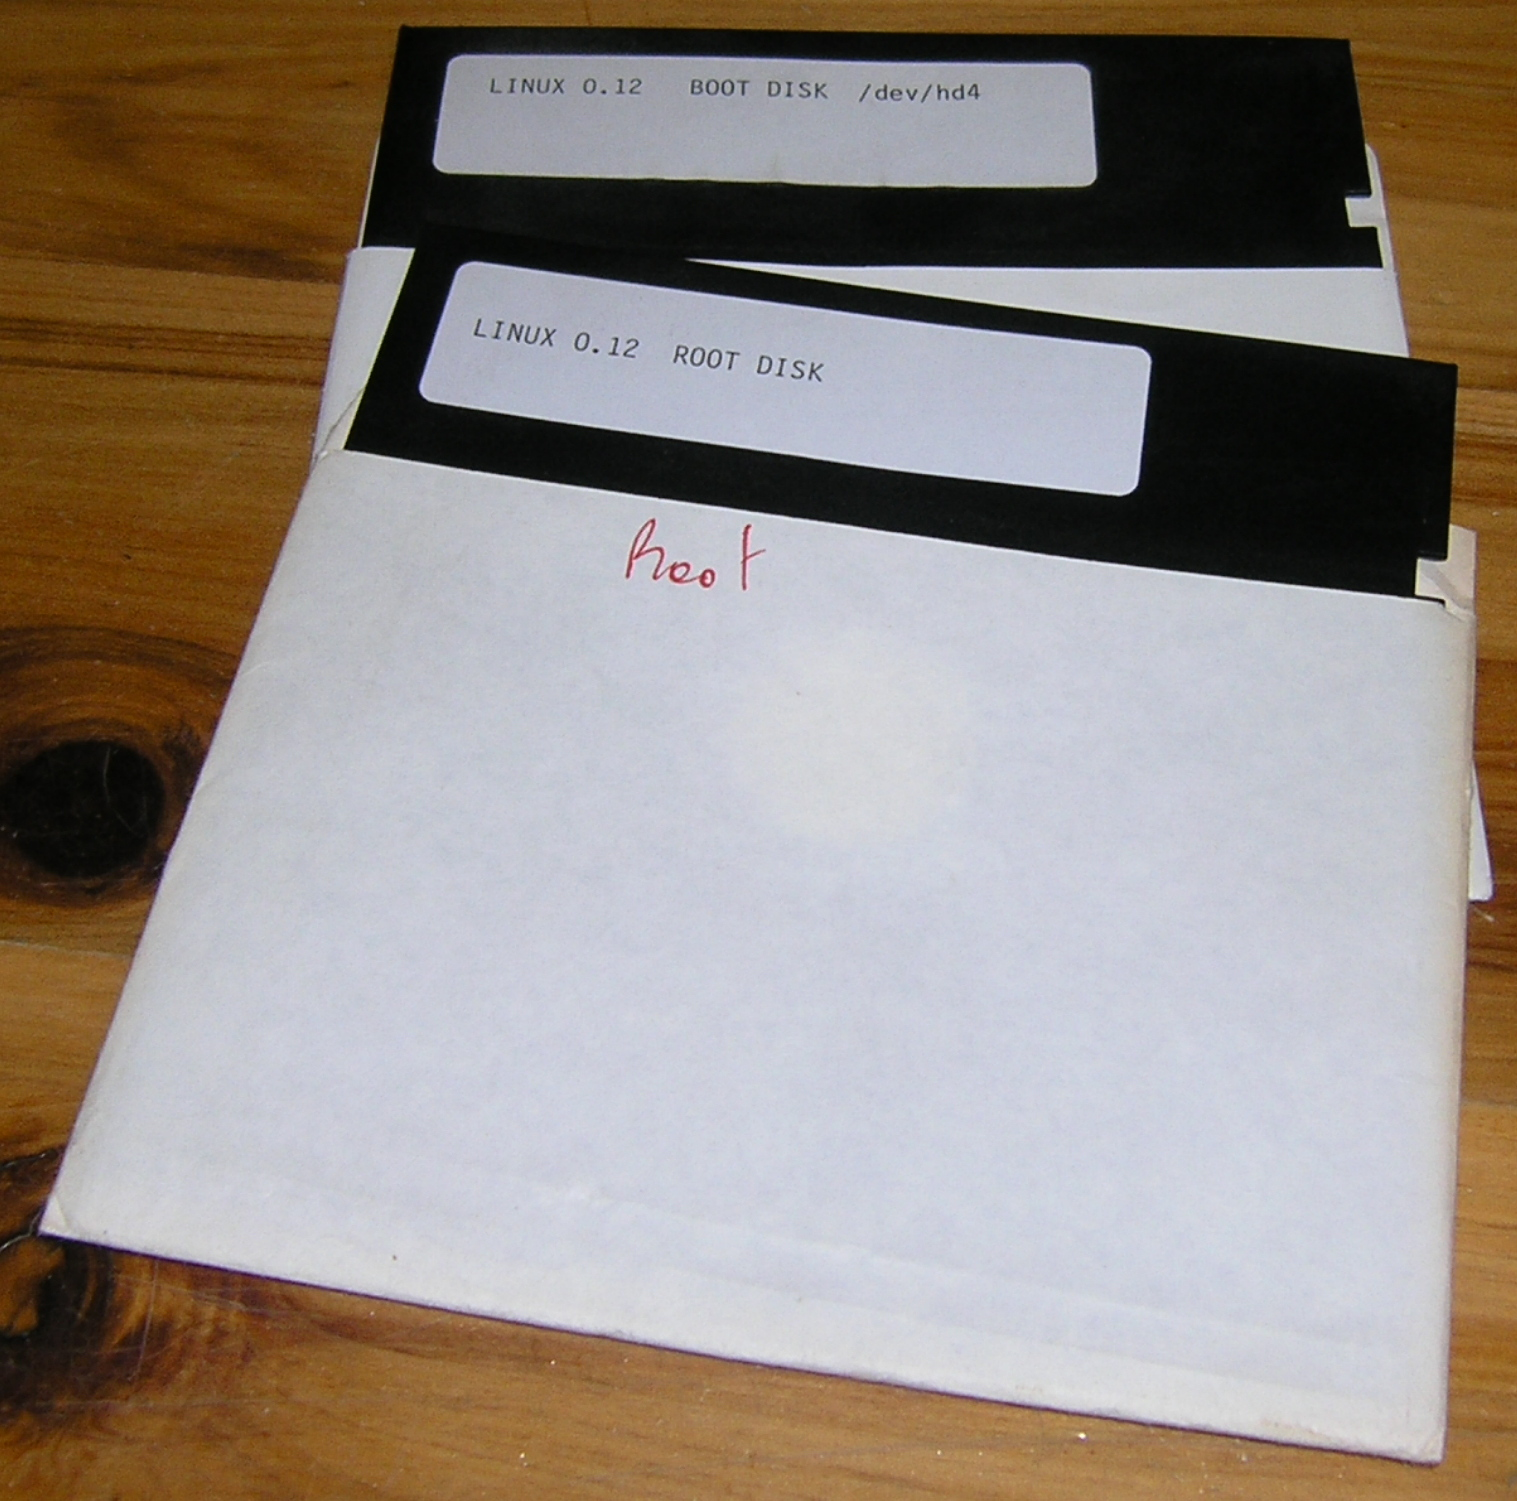
\includegraphics[height=3cm,width=4cm]{old_linux} }}
    \hspace{1cm}
    \subfloat[Ričard Metju Stalman, tvorac GNU-a]{{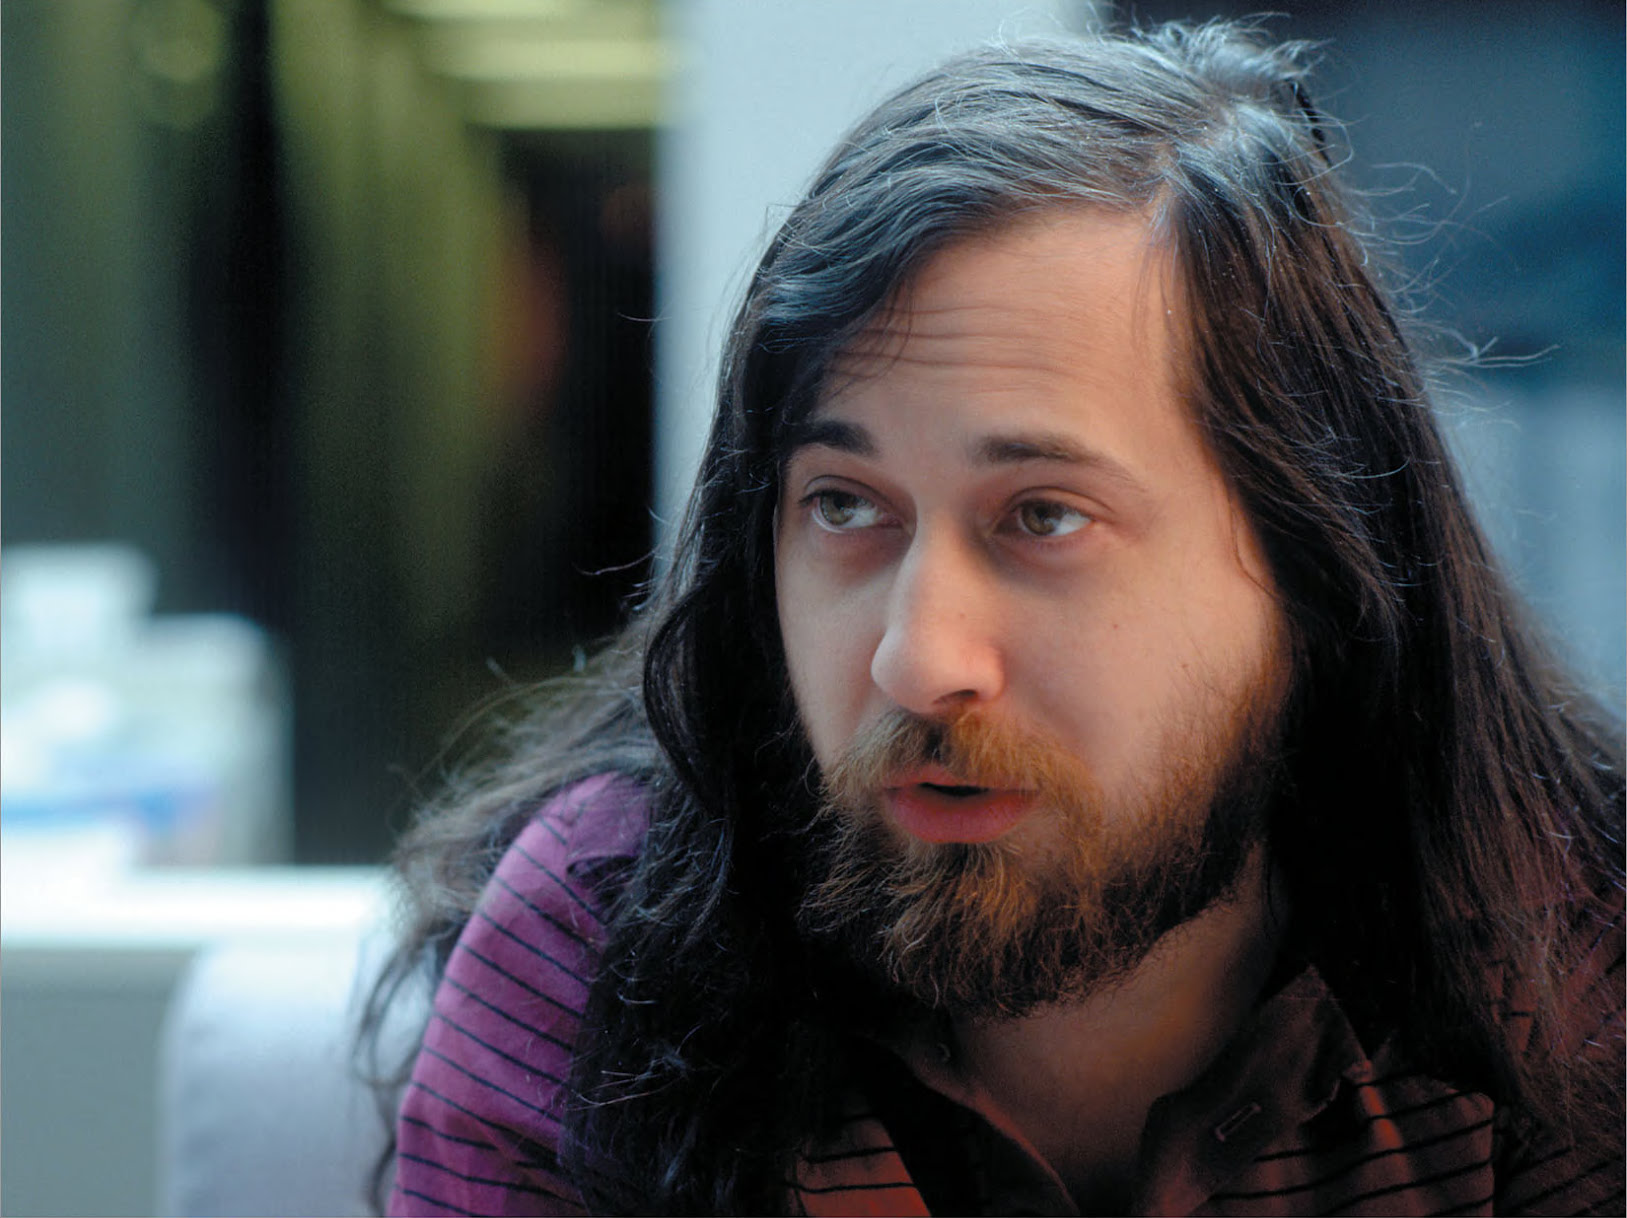
\includegraphics[height=3cm,width=4cm]{stallman} }}
\end{figure}
\begin{figure}[H]
	\centering
	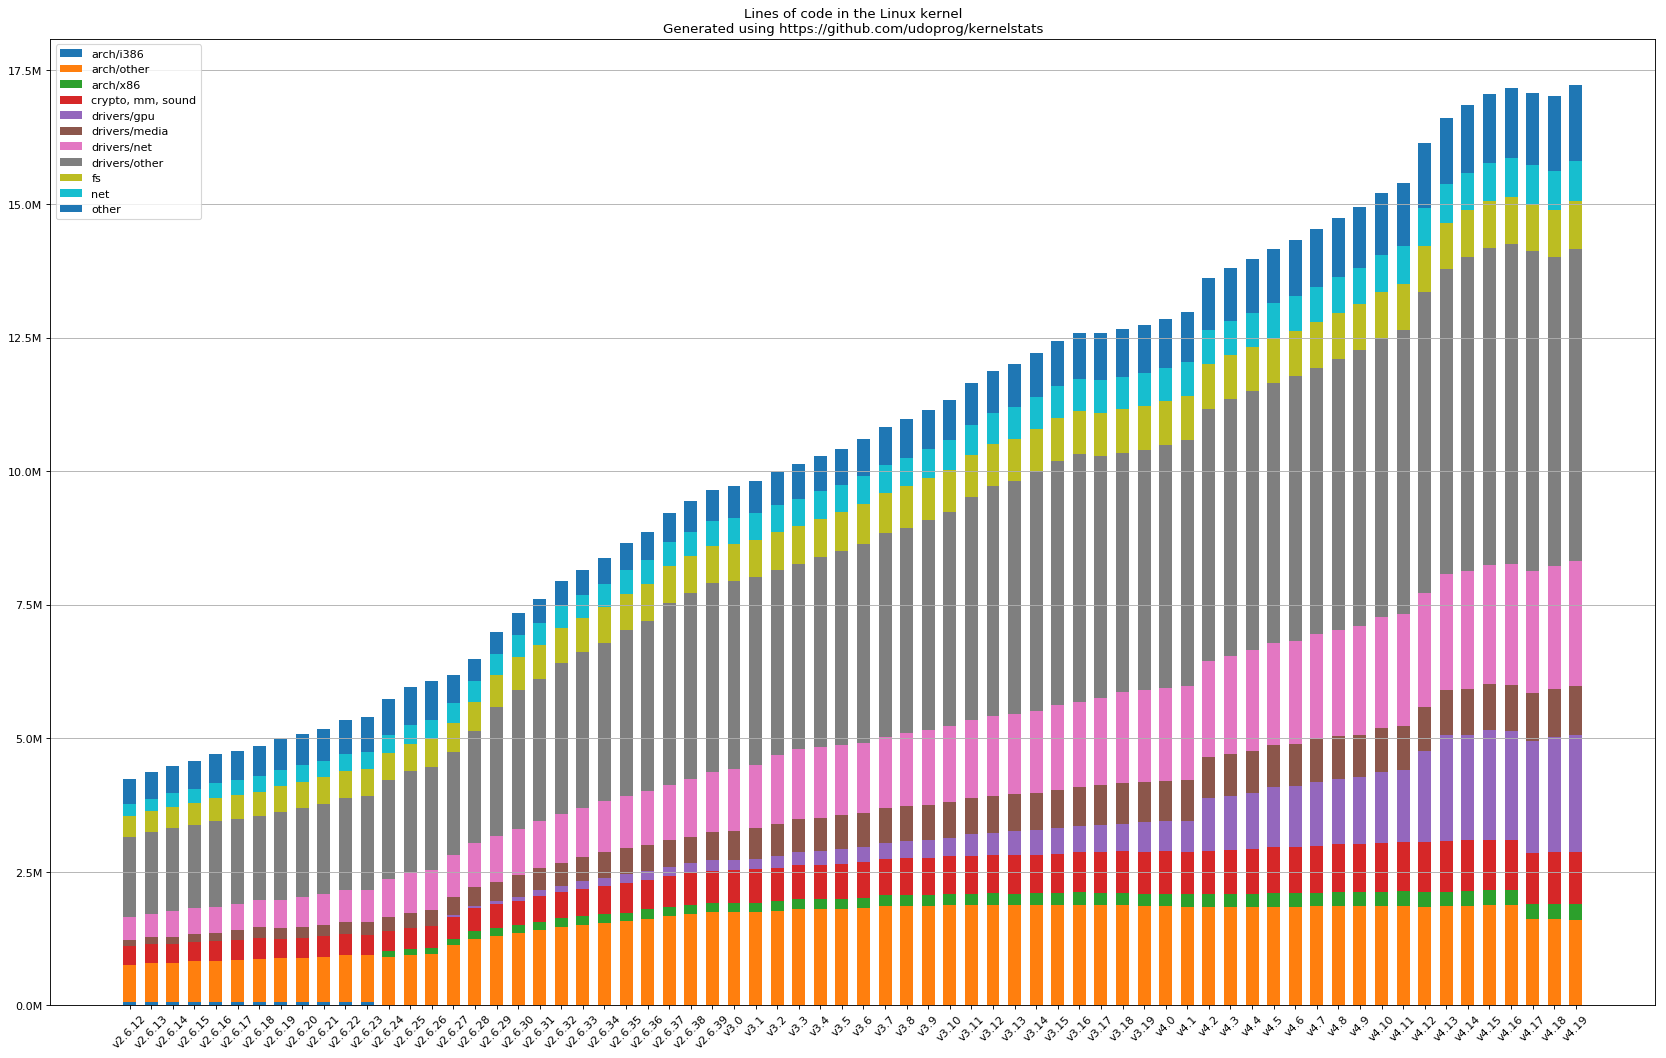
\includegraphics[width=\textwidth]{loc}
	\caption{Broj linija koda u Linux kernel-u od verzije 2.6.12 do danas}
\end{figure}
\newpage

\renewcommand\refname{Literatura}
\bibliographystyle{unsrt}
\addcontentsline{toc}{section}{Literatura}
\bibliography{bib}
\end{document}